\section{Fundamentos de la Educación}

\paragraph{Círculo virtuoso de reflexión en la acción}
La educación es un conocimiento práctico; es un \textit{saber} que consiste en \textit{saber hacer} y que se aprende en el propio \textit{hacer}.
%
Esto suscita una interesante reflexión.
%
Si se aprende haciendo, tras año de experiencia en la profesión, se debería haber acumulado un gran saber.
%
Es bien sabido que esto no ocurre así.
%
Los profesores más veteranos tienen más experiencia pero no necesariamente tienen más dominio del arte de enseñar que los profesores jóvenes. 

Podría darse el caso de que haya profesores que con los años de experiencia hayan ido perdiendo dominio del arte. 
%
Es verdad que hay otras variables tremendamente influyentes en el proceso de mejora y aprendizaje de los profesores, más allá de los años de experiencia.
%
Chojin, en su canción "\textit{Soy y no soy}" hace una afirmación muy acertada: \textit{Cuando aprendo no es por la experiencia en sí sino por el momento que me pille dispuesto y abierto}.
%
Se puede enseñar, pero depende del educando aprender.
%
El aprendizaje y la mejora del educador como docente no depende de sus años de práctica, sino de la actitud dispuesta y abierta a aprender y agrandar el saber hacer.
%
Si el educador no realiza un trabajo de reflexión y evaluación sobre su propia acción educativa, difícilmente va a poder seguir aprendiendo la labor docente.

\begin{figure}[hbt]
\centering
\caption{Círculo de mejora de la acción educativa.}
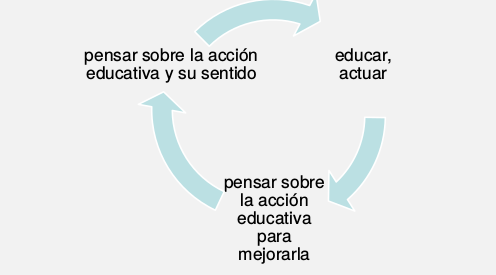
\includegraphics[scale=0.5]{\preffix/img/Circulo.png}

\small{Fuente: Material para las clases de \profe.}
\label{Circulo}
\end{figure}

\paragraph{Educar para ayudar a crecer} A veces confundimos educación con formación. 
%
Es habitual pensar en la educación como el medio para introducirse en un mercado laboral y para ello es necesaria una formación en conocimientos bastante amplia.
%
Poco a poco se va transformando la sociedad en su conjunto hacia un concepto de educación más amplio, más integrador de las diferentes facetas humanas.

"Education is not the learning of facts, but the training of the mind to think" \footnote{En español: La educación no es el aprendizaje de hechos, sino el entrenamiento de la mente para pensar.} es una frase de Einstein.
%
Einstein no hablaba de crecer sino de aprender a pensar. 
%
Una interpretación de esta frase se basa en entender que \textit{pensar} es una acción muy amplia. 
%
De hecho, el crecimiento que se busca en la educación es un crecimiento de las potencias propias (Inteligencia y Voluntad), por lo que, tal vez, Einstein no andaba desencaminado.

Es reconfortante y alentador descubrir que la propuesta educativa dada a los futuros educadores es la que uno traía ya pensada de casa.
%
Es confirmador de la vocación ver que la idea y el sueño de uno para su acción profesional coincida con la de los expertos en la materia.


\subparagraph{Armonía de todas las dimensiones} 
%
Es tremendamente aclaradora la metáfora de la poda.
%
Para forjar el carácter de los educandos es necesario cultivar y dejar crecer, pero puede haber momentos de poda.
%
La poda de una viña, por ejemplo, no quita solamente los sarmientos muertos o los que no dan fruto, sino que también puede interesar cortar sarmientos que dan poco fruto para que vuelvan a crecer más fuertes y fructíferos.

Esta metáfora de la poda resulta interesante. 
%
¿Merecerá la pena un castigo\footnote{Entendiendo castigo desde la definición Psicológica asociada a los refuerzos.} en una situación ambigüa o mediocre para que el educando pueda crecer?



\paragraph{Manipulación} 
%
Este es un tema que se discute poco desde un punto de vista ético y moral.
%
Todas las personas buscan influir en los demás, desde decisiones poco importantes hasta decisiones vitales.
%
¿Quién no ha vivido una situación en la que alguien se estaba equivocando (o eso se pensaba) y se le ha intentado conducir y corregir? 
%
Eso podría estar claro que no es una manipulación ya que se trata por el bien del otro.
%
¿Y si, en esa corrección, el corrector sale beneficiado y busca el cambio de actitud del corregido porque también sale beneficiado?
%
Los límites de la manipulación se difuminan porque es difícil ponderar la importancia que se le está dando al bien de la otra persona y al bien propio.
%
¿Y si busco el bien de un tercero?
%
Como docente podría interesar influir en un determinado estudiante para que modificara su actitud, no tanto por su propio bien personal, sino por el bien de los demás alumnos.
%
¿Quién no ha escuchado "Tu siéntate ahí, calladito y no molestes."?
%
Se están silenciando dimensiones propias de la libertad y no se está buscando el bien para esa persona.
%
¿Es esto una manipulación? ¿Se considera simplemente influencia? ¿Es éticamente correcta?

Como conclusión es importante destacar que, cuando mostramos el fin de una determinada influencia o persuasión, estamos salvaguardándonos de caer en una manipulación.
%
Además, es importante hacer capaz a la otra persona de pensar por sí misma. 



\paragraph{Cuando no educar: Nunca}
Una tentación de la profesión docente es a reducir al ámbito escolar la labor educativa.
%
Si un profesor se encuentra con alumnos por la calle que están realizando un acto de vandalismo, la opción fácil es no educar pasando desapercibido y no interviniendo.
%
Tal vez en un acto vandálico es más fácil intervenir.
%
¿Y si están de botellón? ¿Sería necesario intervenir? 
%
Si hacemos caso a que no se debe no educar nunca, lo ideal sería intervenir.

Un ejemplo menos drástico y más fácil sería a la hora de cruzar la acera. 
%
El docente es educador también fuera del centro escolar y su ejemplo es importante.
%
¿Qué educación ofrece a los alumnos que los profesores crucen mal? 
%
¿O que fumen?
%
Es importante ser ejemplares en todo momento, no sólo en el centro o sus proximidades.




\newpage
\section{Condiciones, elementos y ámbitos para educar}

En este tema se sigue trabajando una idea: el educador no causa el crecimiento del alumno. 
%
El docente sólo pone las condiciones necesarias para que ese crecimiento se pueda dar.

Todos hemos oído y experimentado que el aprecio por parte de los profesores es importante. 
%
Esta idea se ha visto apoyada por investigaciones modernas. 
%
Para que se puedan producir aprendizajes es necesaria la activación de la amígdala cerebral y éste fenómeno se da con mayor intensidad en estados anímicos positivos: cuando el alumno se siente apreciado y aceptado.

El fenómeno de la indefensión aprendida se relaciona mucho con las condiciones de competencia percibida y confianza.

\begin{defn}[Indefensión Aprendida]
Condición de un ser humano o animal que ha aprendido a comportarse pasivamente, con la sensación subjetiva de no poder hacer nada y que no responde a pesar de que existen oportunidades reales de cambiar la situación aversiva, evitando las circunstancias desagradables o mediante la obtención de recompensas positivas.
\end{defn}

Existe la creencia de que este fenómeno se produce con gran frecuencia e intensidad en las aulas de matemáticas. 
%
Decimos creencia porque no se han encontrado investigaciones que lo constaten científicamente.

Es fundamental como profesor conocer que estas condiciones son necesarias para el aprendizaje\footnote{Entendiendo aprendizaje como crecimiento y ejercicio de las potencias racionales o entrenamiento de la mente para \textit{pensar matemáticamente}.} y más fundamentalmente todavía para profesores de matemáticas donde la autocompetencia percibida puede ser muy escasa, con la consiguiente falta de autoconfianza.

\subparagraph{Contribución:} Una condición sorprendente es la de contribuir.
%
Parece instaurado en el sentido común que a los niños y adolescentes más movidos hay que darles responsabilidades para que no se aburran.
%
Pero parece que va más allá: parece que sentirse contribuidor es importante para los alumnos.

Este planteamiento es muy interesante para aulas donde se trabaja con la metodología de aprendizaje cooperativo, ya que hay muchas contribuciones.
%
De hecho, esta condición alerta de un posible peligro. 
%
¿Qué ocurre si uno del grupo no está siendo capaz de contribuir?
%
Será necesario plantear alguna tarea en la que esa persona pueda contribuir o tal vez otorgarle alguna responsabilidad dentro del grupo que sólo ella pueda llevar a cabo.

Por otro lado, para aulas donde no se trabaje cooperativamente ni por proyectos, ¿cómo ofrecer un sentido de contribución a los estudiantes?
%
Tal vez no es una pregunta que se pueda contestar ahora, pero sí es una pregunta a tener en mente para cada ejercicio de reflexión tras la acción docente ejercida.


\paragraph{Límites:} El P. Granda decía a los padres con los que trataba: "Los límites, pocos y bien puestos".
%
Los límites son necesarios pero no hay que sobrelimitar.
%
Hay aspectos en los que es necesario ser tajante, pero hay otros donde se puede ser más laxo.


Un aspecto sorprendente es que los límites fomentan la autonomía.
%
Al establecer con claridad un entorno de seguridad (qué se puede y qué no se puede; cuándo se puede y cuándo no) se permite una amplia libertad sin coacción por el miedo dentro de esas fronteras limitadoras.

Un aspecto de sentido común es que los límites deben ser establecidos y explicados a su debido tiempo, sobretodo con anterioridad a un posible incumplimiento.
%
Este verano, en un campamento de verano, se castigó una actitud (esconder comida en las habitaciones) sin haber especificado con anterioridad que estaba totalmente fuera de los límites mantener comida en las habitaciones.
%
Este castigo provocó el enfado de los acampados, que tuvieron que acabar aceptando y acatando un límite que no se había definido, lo que provocó un cierto deterioro en las relaciones interpersonales.


\newpage
\section{La familia como agente educativo}

Para mi futura labor como docente este tema me ha aportado fundamentalmente 2 aspectos: visión global sobre el papel de la familia y pautas concretas sobre la preparación de las entrevistas.

\subsection{Papel de la familia}

Conocer que el derecho internacional (la declaración de los derechos humanos) establece que \textit{Los padres tienen el derecho preferente a elegir la educación de sus hijos conforme a sus propias convicciones filosóficas y religiosas} resulta novedoso.
%
Esta apartado de la declaración critica regímenes totalitarios en los que la educación religiosa se prohíba (como podría ser la revolución francesa o el comunismo).

Por otro lado, aunque se establezca este derecho, no tiene porqué ejercerse mediante la elección de un centro con un ideario en concreto, sino que debe ir más allá.
%
Los padres siguen siendo los principales responsables de la educación de los hijos también en los ámbitos filosófico y religioso y por tanto no deben delegar totalmente esta función en el centro educativo.
%
No corresponde a otras personas que no sean los padres educar a los hijos según sus propias convicciones.
%
No es labor del centro reeducar a los hijos según sus convicciones, sino apoyar a los padres.

Esto es aplicable tanto a docentes que creen que su labor pasa por contrarrestar las convicciones religiosas de los padres bajo el argumento de que sea el hijo quien elija, como a los docentes que creen que su labor consiste en educar a los hijos en unas convicciones morales, religiosas y filosóficas contrarias a las de los padres.

Aunque todavía no he tengo respuesta a este conflicto, me ha resultado esclarecedor conocer la normativa internacional y poder reflexionar sobre el tema, ya que es un tema, en mi opinión, bastante enquistado en la sociedad española.
%
Hay quienes están a favor de que todos los centros sean exactamente iguales, laicos, etc. y quienes creemos en la necesidad de diversidad en los idearios de los centros, pero, ante todo, dentro del marco legal de actuación.

\subsection{Preparación de las entrevistas}

Aunque muchas de las cosas explicadas ya las tenía incorporadas en mi repertorio de actuación por el sentido común (como sería preparar una entrevista y tener claros los objetivos de la misma o tener entrevistas para hablar sobre la educación del alumno, aunque no haya surgido ningún problema), han habido algunos otros aspectos que me han resultado muy útiles.

Por ejemplo, volver a pensar en la importancia de realizar una evaluación y una reflexión al final de la acción educativa.
%
Al final de toda acción educativa (como veíamos anteriormente) es fundamental realizar una labor de introspección y reflexión; y esta práctica también incluye la realización de las entrevistas.

Además, es importante tener entrevistas en los tiempos y momentos establecidos.
%
La posibilidad de cruzarse con los padres a la salida del colegio y ahí tratar algunos temas no debería ser contemplada.
%
Tal vez hay algún tema que sí se podría tratar en ese momento, pero no es la manera de tener una entrevista.
%
No permite plantear objetivos de la entrevista, ni seguir una estructura planificada...
%
Lo ideal es tener entrevistas como entrevistas y no como charlas informales en el patio del colegio.
%
Así, ante el avasallamiento de una familia en el patio, la respuesta del docente podría ser: "Este no es el lugar ni el momento para hablar esto. ¿Porqué no te vienes un día y tenemos tranquilamente una tutoría?"




\newpage
\section{Amistad}


Por la labor que realizo en mi tiempo libre en la que tengo mucho contacto con adolescentes, partes de este tema me resultan muy familiares.
%
Sobretodo la dimensión psicológica de la amistad: 
%
he vivido de cerca \textit{crisis} de grupos de amigos adolescentes y he visto la importancia que le dan y el sufrimiento que les genera.
%
También he podido participar en la educación en la amistad fomentando relaciones de calidad, en las que se prioricen aspectos importantes y no banales de la relación; fomentando que se asuma el compromiso que supone una relación, buscando los momentos buenos pero sin huir ni escapar de los malos.

Debido a la escasez de tiempo en la exposición de este tema, hay algunas dudas que me han surgido durante mi trabajo con adolescentes pero que no he sabido resolver todavía.
%
¿Cómo tratar eficazmente con un adolescente que ha tenido un problema con sus amigos y le genera un gran sufrimiento?
%
¿Cómo gestionar los conflictos que surgen entre personas que empezaron a ser amigas con 6 años, pero que al alcanzar los 16 son realmente muy distintas y no hay manera de que se lleven bien? 
%
¿Cómo ayudar a diferenciar amistad de algo más?
%
¿Cómo tratar los conflictos cunado una de las 2 partes confunde amistad con algo más, o incluso siente la amistad como algo más, y la otra no?

Por otro lado, me ha resultado muy reforzador conocer que desde el punto de vista teórico se estudian y establecen conclusiones a las que había llegado desde mi experiencia.
%
Ahora sé que algunas de las cosas que yo pensaba son extrapolables a otras situaciones con otras personas, porque desde la investigación se confirman.

Como conclusión, para mi vida personal más que para mi labor docente, me quedo con que el modelo familiar que los hijos ven es el que aplican.
%
En mi familia siempre hemos tenido un póster que decía "Los niños aprenden lo que viven" (ver figura \ref{img:ninos})
%
Este tema me ha hecho reflexionar también sobre lo siguiente:
%
los alumnos también pueden aprender de las relaciones que yo mantenga con mis amigos y que ellos vean, ya sean las relaciones entre profesores como las relaciones con mi comunidad que algunos de ellos ven de vez en cuando.
%
Creo que yo también soy un modelo de referencia para ellos (de menor peso, obviamente, que la familia) y tengo que tenerlo en cuenta.
%
Además, si acabo formando una familia será importante que las relaciones que mantenga sean ejemplares, por mi bien y el de mis hijos e hijas.


\begin{figure}[hbtp]
\centering
\caption{Póster que siempre ha estado colgado en la cocina de mi casa.}
\label{img:ninos}
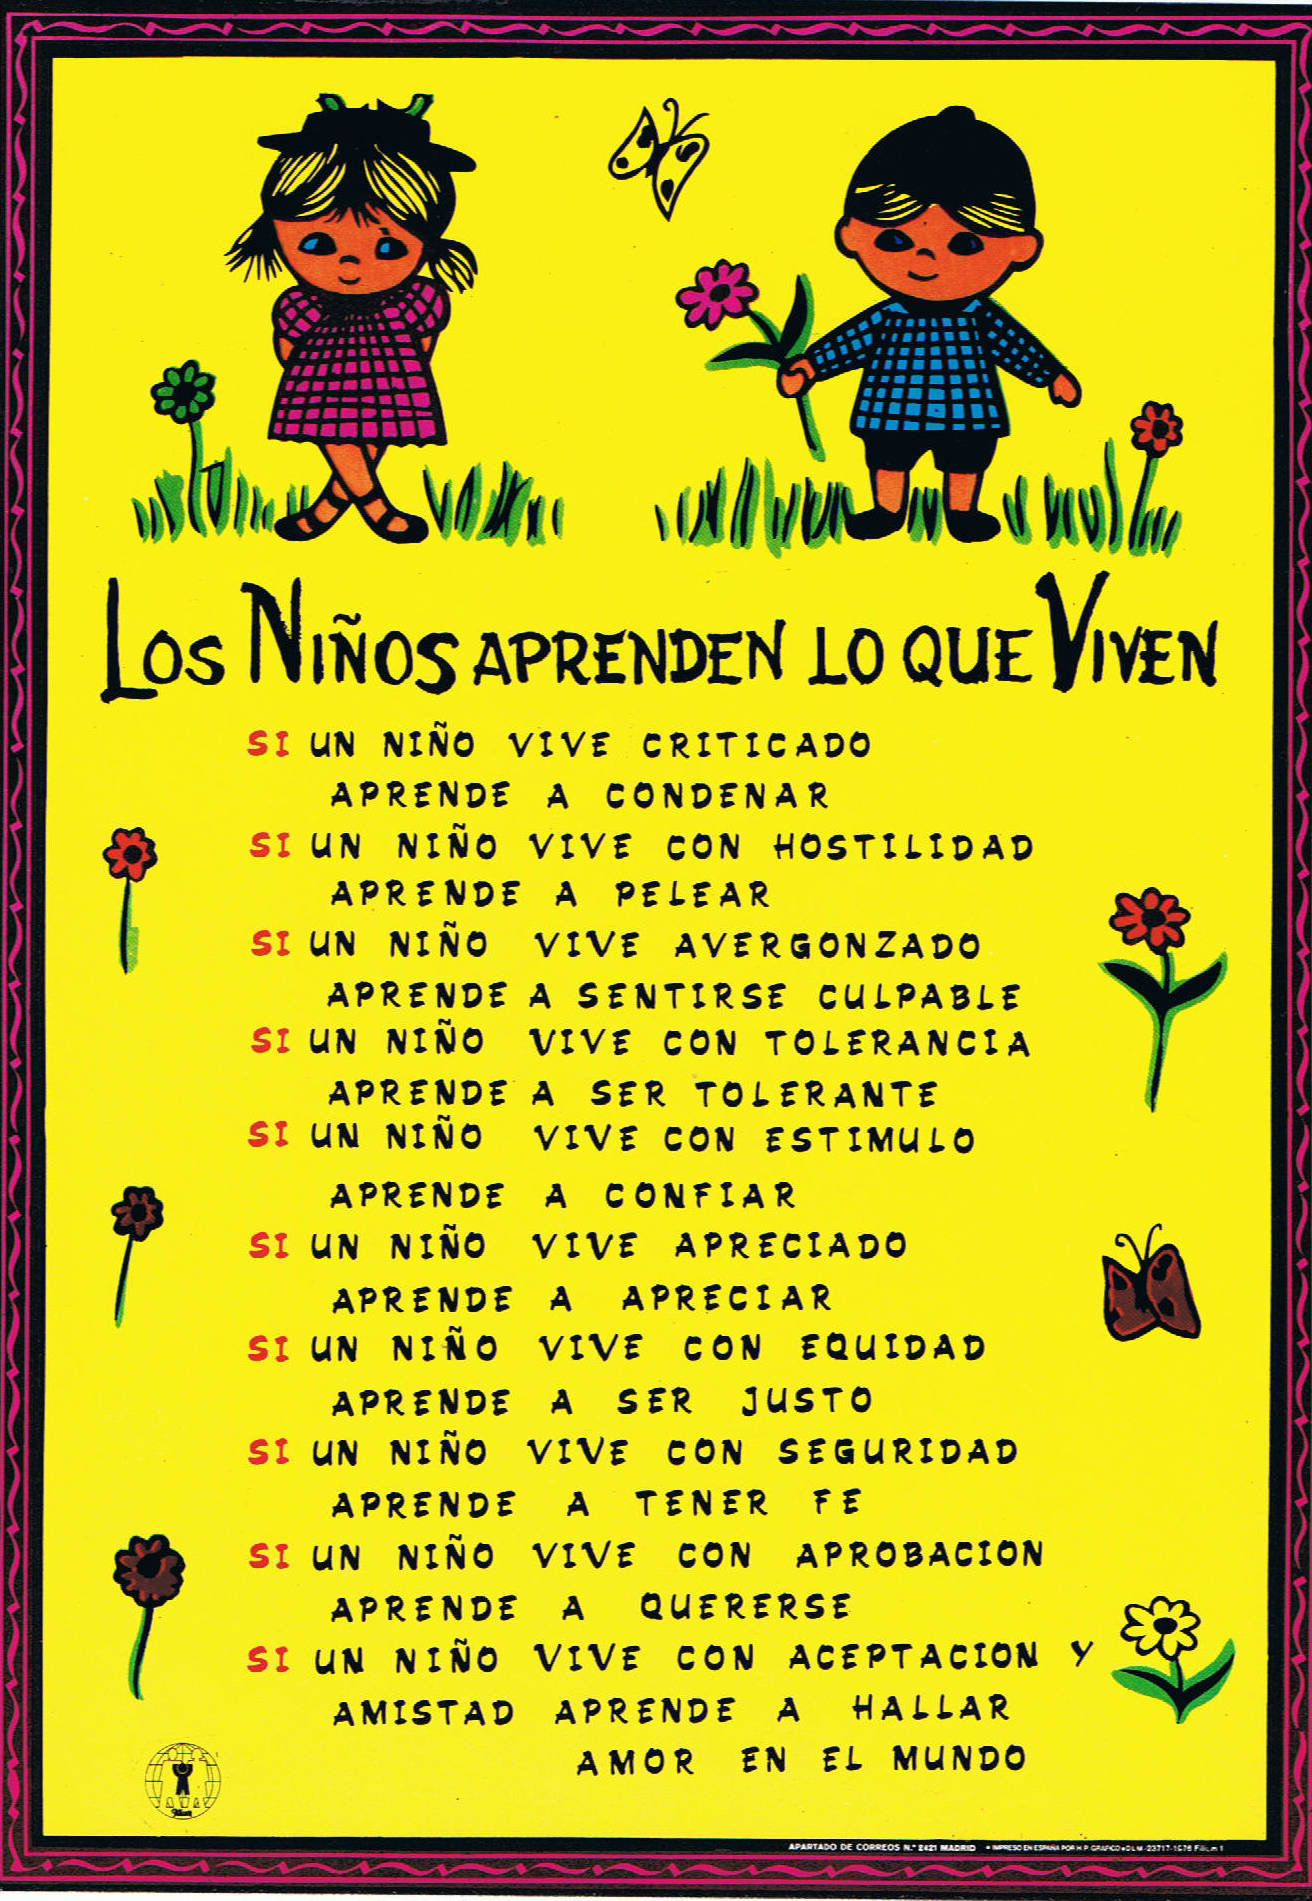
\includegraphics[scale=0.3]{\preffix/img/ninos.jpg}

\small{Fuente: \href{https://www.terapia-psicored-cam.com/psicoanalistas-articulos?lightbox=image3ht}{terapia-psicored-cam.com}}
\end{figure}


